\documentclass[11pt,compress,t,notes=noshow, xcolor=table]{beamer}
\usepackage[]{graphicx}
\usepackage[]{color}
% maxwidth is the original width if it is less than linewidth
% otherwise use linewidth (to make sure the graphics do not exceed the margin)
\makeatletter
\def\maxwidth{ %
  \ifdim\Gin@nat@width>\linewidth
    \linewidth
  \else
    \Gin@nat@width
  \fi
}
\makeatother

% ---------------------------------%
% latex-math dependencies, do not remove:
% - \usepackage{mathtools}
% - \usepackage{bm}
% - \usepackage{siunitx}
% - \usepackage{dsfont}
% - \usepackage{xspace}
% ---------------------------------%

%--------------------------------------------------------%
%       Language, encoding, typography
%--------------------------------------------------------%

\usepackage[english]{babel}
\usepackage[utf8]{inputenc} % Enables inputting UTF-8 symbols
% Standard AMS suite
\usepackage{amsmath,amsfonts,amssymb}

% Font four double-stroke / blackboard letters for sets of numbers (N, R, ...)
% Distribution name is "doublestroke"
% According to https://mirror.physik.tu-berlin.de/pub/CTAN/fonts/doublestroke/dsdoc.pdf
% the "bbm" package does a similar thing and may be superfluous.
% Required for latex-math
\usepackage{dsfont}

% bbm – "Blackboard-style" cm fonts (https://www.ctan.org/pkg/bbm)
% Used to be in common.tex, loaded directly after this file
% Maybe superfluous given dsfont is loaded
% TODO: Check if really unused?
% \usepackage{bbm}

% bm – Access bold symbols in maths mode - https://ctan.org/pkg/bm
% Required for latex-math
% https://tex.stackexchange.com/questions/3238/bm-package-versus-boldsymbol
\usepackage{bm}

% pifont – Access to PostScript standard Symbol and Dingbats fonts
% Used for \newcommand{\xmark}{\ding{55}, which is never used
% aside from lecture_advml/attic/xx-automl/slides.Rnw
% \usepackage{pifont}

% Quotes (inline and display), provdes \enquote
% https://ctan.org/pkg/csquotes
\usepackage{csquotes}

% Adds arg to enumerate env, technically superseded by enumitem according
% to https://ctan.org/pkg/enumerate
% Replace with https://ctan.org/pkg/enumitem ?
\usepackage{enumerate}

% Line spacing - provides \singlespacing \doublespacing \onehalfspacing
% https://ctan.org/pkg/setspace
% TODO: Check if really unused?
%\usepackage{setspace}

% mathtools – Mathematical tools to use with amsmath
% https://ctan.org/pkg/mathtools?lang=en
% latex-math dependency according to latex-math repo
\usepackage{mathtools}

%--------------------------------------------------------%
%       Displaying code and algorithms
%--------------------------------------------------------%
\usepackage{verbatim}
\usepackage{algorithm}
\usepackage{algpseudocode}

%--------------------------------------------------------%
%       Tables
%--------------------------------------------------------%

% multi-row table cells: https://www.namsu.de/Extra/pakete/Multirow.html
\usepackage{multirow}

% long/multi-page tables: https://texdoc.org/serve/longtable.pdf/0
% TODO: Check if really unused?

\usepackage{longtable}

% pretty table env: https://ctan.org/pkg/booktabs?lang=en
% TODO: Check if really unused?
\usepackage{booktabs}

%--------------------------------------------------------%
%       Figures: Creating, placing, verbing
%--------------------------------------------------------%

% wrapfig - Wrapping text around figures https://de.overleaf.com/learn/latex/Wrapping_text_around_figures
\usepackage{wrapfig}

% Sub figures in figures and tables
% https://ctan.org/pkg/subfig -- supersedes subfigure package
% TODO: Check if really unused?
\usepackage{subfig}

% Actually it's pronounced PGF https://en.wikibooks.org/wiki/LaTeX/PGF/TikZ
\usepackage{tikz}

\usetikzlibrary{shapes,arrows,automata,positioning,calc,chains,trees, shadows}
\tikzset{
  %Define standard arrow tip
  >=stealth',
  %Define style for boxes
  punkt/.style={
    rectangle,
    rounded corners,
    draw=black, very thick,
    text width=6.5em,
    minimum height=2em,
    text centered},
  % Define arrow style
  pil/.style={
    ->,
    thick,
    shorten <=2pt,
    shorten >=2pt,}
}


% Unsorted
% textpos – Place boxes at arbitrary positions on the LATEX page
% https://ctan.org/pkg/textpos?lang=en
% Provides \begin{textblock}
 % TODO: Check if really unused?
\usepackage[absolute,overlay]{textpos}

% psfrag – Replace strings in encapsulated PostScript figures
% https://www.overleaf.com/latex/examples/psfrag-example/tggxhgzwrzhn
% https://ftp.mpi-inf.mpg.de/pub/tex/mirror/ftp.dante.de/pub/tex/macros/latex/contrib/psfrag/pfgguide.pdf
% Can't tell if this is needed
% TODO: Check if really unused?
\usepackage{psfrag}

% Maybe not great to use this https://tex.stackexchange.com/a/197/19093
% Use align instead -- TODO: Global search & replace to check
\usepackage{eqnarray}

\usepackage{colortbl}

% arydshln – Draw dash-lines in array/tabular
% https://www.ctan.org/pkg/arydshln
% !! "arydshln has to be loaded after array, longtable, colortab and/or colortbl"
% Provides \hdashline and \cdashline
% TODO: Check if really unused?
% \usepackage{arydshln}

% tabularx – Tabulars with adjustable-width columns
% https://ctan.org/pkg/tabularx
% Provides \begin{tabularx}
% TODO: Check if really unused?
% \usepackage{tabularx}

% placeins – Control float placement
% https://ctan.org/pkg/placeins
% Defines a \FloatBarrier command
% TODO: Check if really unused?
% \usepackage{placeins}


% framed – Framed or shaded regions that can break across pages
% https://ctan.org/pkg/framed
% Provides \begin{framed} which uses \colorbox{shadecolor} relying on \definecolor{shadecolor}.
% TODO: Check if really unused?
% \usepackage{framed}

% Used often in conjunction with \definecolor{shadecolor}{rgb}{0.969, 0.969, 0.969}
% Might be able to be removed or at least redefined to only have shadecolor (if needed)
\definecolor{fgcolor}{rgb}{0.345, 0.345, 0.345}
\definecolor{shadecolor}{rgb}{0.969, 0.969, 0.969}
\newenvironment{knitrout}{}{} % an empty environment to be redefined in TeX


% Defines macros and environments
\usepackage{../../style/lmu-lecture}

\let\code=\texttt % Used regularly
\let\proglang=\textsf % Unused?

% Not sure what/why this does
\setkeys{Gin}{width=0.9\textwidth}

\setbeamertemplate{frametitle}{\expandafter\uppercase\expandafter\insertframetitle}

% Can't find a reason why common.tex is not just part of this file?
% Rarely used fontstyle for R packages, used only in 
% - forests/slides-forests-benchmark.tex
% - exercises/single-exercises/methods_l_1.Rnw
% - slides/cart/attic/slides_extra_trees.Rnw
\newcommand{\pkg}[1]{{\fontseries{b}\selectfont #1}}

% Spacing helpers, used often (mostly in exercises for \dlz)
\newcommand{\lz}{\vspace{0.5cm}} % vertical space (used often in slides)
\newcommand{\dlz}{\vspace{1cm}}  % double vertical space (used often in exercises, never in slides)

%--------------------%
%  New environments  %
%--------------------%

 % Frame with breaks and verbatim // this is used very often
\newenvironment{vbframe}
{
\begin{frame}[containsverbatim,allowframebreaks]
}
{
\end{frame}
}

% Frame with verbatim without breaks (to avoid numbering one slided frames)
% This is not used anywhere but I can see it being useful
\newenvironment{vframe}
{
\begin{frame}[containsverbatim]
}
{
\end{frame}
}

% Itemize block
\newenvironment{blocki}[1]
{
\begin{block}{#1}\begin{itemize}
}
{
\end{itemize}\end{block}
}

% textcolor that works in mathmode
% https://tex.stackexchange.com/a/261480
% Used e.g. in forests/slides-forests-bagging.tex
% [...] \textcolor{blue}{\tfrac{1}{M}\sum^M_{m} [...]
% \makeatletter
% \renewcommand*{\@textcolor}[3]{%
%   \protect\leavevmode
%   \begingroup
%     \color#1{#2}#3%
%   \endgroup
% }
% \makeatother


%-------------------------------------------------------------------------------------------------------%
%  Unused stuff that needs to go but is kept here currently juuuust in case it was important after all  %
%-------------------------------------------------------------------------------------------------------%

% \newcommand{\hlnum}[1]{\textcolor[rgb]{0.686,0.059,0.569}{#1}}%
% \newcommand{\hlstr}[1]{\textcolor[rgb]{0.192,0.494,0.8}{#1}}%
% \newcommand{\hlcom}[1]{\textcolor[rgb]{0.678,0.584,0.686}{\textit{#1}}}%
% \newcommand{\hlopt}[1]{\textcolor[rgb]{0,0,0}{#1}}%
% \newcommand{\hlstd}[1]{\textcolor[rgb]{0.345,0.345,0.345}{#1}}%
% \newcommand{\hlkwa}[1]{\textcolor[rgb]{0.161,0.373,0.58}{\textbf{#1}}}%
% \newcommand{\hlkwb}[1]{\textcolor[rgb]{0.69,0.353,0.396}{#1}}%
% \newcommand{\hlkwc}[1]{\textcolor[rgb]{0.333,0.667,0.333}{#1}}%
% \newcommand{\hlkwd}[1]{\textcolor[rgb]{0.737,0.353,0.396}{\textbf{#1}}}%
% \let\hlipl\hlkwb

% \makeatletter
% \newenvironment{kframe}{%
%  \def\at@end@of@kframe{}%
%  \ifinner\ifhmode%
%   \def\at@end@of@kframe{\end{minipage}}%
%   \begin{minipage}{\columnwidth}%
%  \fi\fi%
%  \def\FrameCommand##1{\hskip\@totalleftmargin \hskip-\fboxsep
%  \colorbox{shadecolor}{##1}\hskip-\fboxsep
%      % There is no \\@totalrightmargin, so:
%      \hskip-\linewidth \hskip-\@totalleftmargin \hskip\columnwidth}%
%  \MakeFramed {\advance\hsize-\width
%    \@totalleftmargin\z@ \linewidth\hsize
%    \@setminipage}}%
%  {\par\unskip\endMakeFramed%
%  \at@end@of@kframe}
% \makeatother

% \definecolor{shadecolor}{rgb}{.97, .97, .97}
% \definecolor{messagecolor}{rgb}{0, 0, 0}
% \definecolor{warningcolor}{rgb}{1, 0, 1}
% \definecolor{errorcolor}{rgb}{1, 0, 0}
% \newenvironment{knitrout}{}{} % an empty environment to be redefined in TeX

% \usepackage{alltt}
% \newcommand{\SweaveOpts}[1]{}  % do not interfere with LaTeX
% \newcommand{\SweaveInput}[1]{} % because they are not real TeX commands
% \newcommand{\Sexpr}[1]{}       % will only be parsed by R
% \newcommand{\xmark}{\ding{55}}%

% dependencies: amsmath, amssymb, dsfont
% math spaces
\ifdefined\N
\renewcommand{\N}{\mathds{N}} % N, naturals
\else \newcommand{\N}{\mathds{N}} \fi
\newcommand{\Z}{\mathds{Z}} % Z, integers
\newcommand{\Q}{\mathds{Q}} % Q, rationals
\newcommand{\R}{\mathds{R}} % R, reals
\ifdefined\C
\renewcommand{\C}{\mathds{C}} % C, complex
\else \newcommand{\C}{\mathds{C}} \fi
\newcommand{\continuous}{\mathcal{C}} % C, space of continuous functions
\newcommand{\M}{\mathcal{M}} % machine numbers
\newcommand{\epsm}{\epsilon_m} % maximum error

% counting / finite sets
\newcommand{\setzo}{\{0, 1\}} % set 0, 1
\newcommand{\setmp}{\{-1, +1\}} % set -1, 1
\newcommand{\unitint}{[0, 1]} % unit interval

% basic math stuff
\newcommand{\xt}{\tilde x} % x tilde
\DeclareMathOperator*{\argmax}{arg\,max} % argmax
\DeclareMathOperator*{\argmin}{arg\,min} % argmin
\newcommand{\argminlim}{\mathop{\mathrm{arg\,min}}\limits} % argmax with limits
\newcommand{\argmaxlim}{\mathop{\mathrm{arg\,max}}\limits} % argmin with limits
\newcommand{\sign}{\operatorname{sign}} % sign, signum
\newcommand{\I}{\mathbb{I}} % I, indicator
\newcommand{\order}{\mathcal{O}} % O, order
\newcommand{\bigO}{\mathcal{O}} % Big-O Landau
\newcommand{\littleo}{{o}} % Little-o Landau
\newcommand{\pd}[2]{\frac{\partial{#1}}{\partial #2}} % partial derivative
\newcommand{\floorlr}[1]{\left\lfloor #1 \right\rfloor} % floor
\newcommand{\ceillr}[1]{\left\lceil #1 \right\rceil} % ceiling
\newcommand{\indep}{\perp \!\!\! \perp} % independence symbol

% sums and products
\newcommand{\sumin}{\sum\limits_{i=1}^n} % summation from i=1 to n
\newcommand{\sumim}{\sum\limits_{i=1}^m} % summation from i=1 to m
\newcommand{\sumjn}{\sum\limits_{j=1}^n} % summation from j=1 to p
\newcommand{\sumjp}{\sum\limits_{j=1}^p} % summation from j=1 to p
\newcommand{\sumik}{\sum\limits_{i=1}^k} % summation from i=1 to k
\newcommand{\sumkg}{\sum\limits_{k=1}^g} % summation from k=1 to g
\newcommand{\sumjg}{\sum\limits_{j=1}^g} % summation from j=1 to g
\newcommand{\meanin}{\frac{1}{n} \sum\limits_{i=1}^n} % mean from i=1 to n
\newcommand{\meanim}{\frac{1}{m} \sum\limits_{i=1}^m} % mean from i=1 to n
\newcommand{\meankg}{\frac{1}{g} \sum\limits_{k=1}^g} % mean from k=1 to g
\newcommand{\prodin}{\prod\limits_{i=1}^n} % product from i=1 to n
\newcommand{\prodkg}{\prod\limits_{k=1}^g} % product from k=1 to g
\newcommand{\prodjp}{\prod\limits_{j=1}^p} % product from j=1 to p

% linear algebra
\newcommand{\one}{\bm{1}} % 1, unitvector
\newcommand{\zero}{\mathbf{0}} % 0-vector
\newcommand{\id}{\bm{I}} % I, identity
\newcommand{\diag}{\operatorname{diag}} % diag, diagonal
\newcommand{\trace}{\operatorname{tr}} % tr, trace
\newcommand{\spn}{\operatorname{span}} % span
\newcommand{\scp}[2]{\left\langle #1, #2 \right\rangle} % <.,.>, scalarproduct
\newcommand{\mat}[1]{\begin{pmatrix} #1 \end{pmatrix}} % short pmatrix command
\newcommand{\Amat}{\mathbf{A}} % matrix A
\newcommand{\Deltab}{\mathbf{\Delta}} % error term for vectors

% basic probability + stats
\renewcommand{\P}{\mathds{P}} % P, probability
\newcommand{\E}{\mathds{E}} % E, expectation
\newcommand{\var}{\mathsf{Var}} % Var, variance
\newcommand{\cov}{\mathsf{Cov}} % Cov, covariance
\newcommand{\corr}{\mathsf{Corr}} % Corr, correlation
\newcommand{\normal}{\mathcal{N}} % N of the normal distribution
\newcommand{\iid}{\overset{i.i.d}{\sim}} % dist with i.i.d superscript
\newcommand{\distas}[1]{\overset{#1}{\sim}} % ... is distributed as ...

% machine learning
\newcommand{\Xspace}{\mathcal{X}} % X, input space
\newcommand{\Yspace}{\mathcal{Y}} % Y, output space
\newcommand{\Zspace}{\mathcal{Z}} % Space of sampled datapoints ! Also defined identically in ml-online.tex !
\newcommand{\nset}{\{1, \ldots, n\}} % set from 1 to n
\newcommand{\pset}{\{1, \ldots, p\}} % set from 1 to p
\newcommand{\gset}{\{1, \ldots, g\}} % set from 1 to g
\newcommand{\Pxy}{\mathbb{P}_{xy}} % P_xy
\newcommand{\Exy}{\mathbb{E}_{xy}} % E_xy: Expectation over random variables xy
\newcommand{\xv}{\mathbf{x}} % vector x (bold)
\newcommand{\xtil}{\tilde{\mathbf{x}}} % vector x-tilde (bold)
\newcommand{\yv}{\mathbf{y}} % vector y (bold)
\newcommand{\xy}{(\xv, y)} % observation (x, y)
\newcommand{\xvec}{\left(x_1, \ldots, x_p\right)^\top} % (x1, ..., xp)
\newcommand{\Xmat}{\mathbf{X}} % Design matrix
\newcommand{\allDatasets}{\mathds{D}} % The set of all datasets
\newcommand{\allDatasetsn}{\mathds{D}_n}  % The set of all datasets of size n
\newcommand{\D}{\mathcal{D}} % D, data
\newcommand{\Dn}{\D_n} % D_n, data of size n
\newcommand{\Dtrain}{\mathcal{D}_{\text{train}}} % D_train, training set
\newcommand{\Dtest}{\mathcal{D}_{\text{test}}} % D_test, test set
\newcommand{\xyi}[1][i]{\left(\xv^{(#1)}, y^{(#1)}\right)} % (x^i, y^i), i-th observation
\newcommand{\Dset}{\left( \xyi[1], \ldots, \xyi[n]\right)} % {(x1,y1)), ..., (xn,yn)}, data
\newcommand{\defAllDatasetsn}{(\Xspace \times \Yspace)^n} % Def. of the set of all datasets of size n
\newcommand{\defAllDatasets}{\bigcup_{n \in \N}(\Xspace \times \Yspace)^n} % Def. of the set of all datasets
\newcommand{\xdat}{\left\{ \xv^{(1)}, \ldots, \xv^{(n)}\right\}} % {x1, ..., xn}, input data
\newcommand{\ydat}{\left\{ \yv^{(1)}, \ldots, \yv^{(n)}\right\}} % {y1, ..., yn}, input data
\newcommand{\yvec}{\left(y^{(1)}, \hdots, y^{(n)}\right)^\top} % (y1, ..., yn), vector of outcomes
\renewcommand{\xi}[1][i]{\xv^{(#1)}} % x^i, i-th observed value of x
\newcommand{\yi}[1][i]{y^{(#1)}} % y^i, i-th observed value of y
\newcommand{\xivec}{\left(x^{(i)}_1, \ldots, x^{(i)}_p\right)^\top} % (x1^i, ..., xp^i), i-th observation vector
\newcommand{\xj}{\xv_j} % x_j, j-th feature
\newcommand{\xjvec}{\left(x^{(1)}_j, \ldots, x^{(n)}_j\right)^\top} % (x^1_j, ..., x^n_j), j-th feature vector
\newcommand{\phiv}{\mathbf{\phi}} % Basis transformation function phi
\newcommand{\phixi}{\mathbf{\phi}^{(i)}} % Basis transformation of xi: phi^i := phi(xi)

%%%%%% ml - models general
\newcommand{\lamv}{\bm{\lambda}} % lambda vector, hyperconfiguration vector
\newcommand{\Lam}{\bm{\Lambda}}	 % Lambda, space of all hpos
% Inducer / Inducing algorithm
\newcommand{\preimageInducer}{\left(\defAllDatasets\right)\times\Lam} % Set of all datasets times the hyperparameter space
\newcommand{\preimageInducerShort}{\allDatasets\times\Lam} % Set of all datasets times the hyperparameter space
% Inducer / Inducing algorithm
\newcommand{\ind}{\mathcal{I}} % Inducer, inducing algorithm, learning algorithm

% continuous prediction function f
\newcommand{\ftrue}{f_{\text{true}}}  % True underlying function (if a statistical model is assumed)
\newcommand{\ftruex}{\ftrue(\xv)} % True underlying function (if a statistical model is assumed)
\newcommand{\fx}{f(\xv)} % f(x), continuous prediction function
\newcommand{\fdomains}{f: \Xspace \rightarrow \R^g} % f with domain and co-domain
\newcommand{\Hspace}{\mathcal{H}} % hypothesis space where f is from
\newcommand{\fbayes}{f^{\ast}} % Bayes-optimal model
\newcommand{\fxbayes}{f^{\ast}(\xv)} % Bayes-optimal model
\newcommand{\fkx}[1][k]{f_{#1}(\xv)} % f_j(x), discriminant component function
\newcommand{\fh}{\hat{f}} % f hat, estimated prediction function
\newcommand{\fxh}{\fh(\xv)} % fhat(x)
\newcommand{\fxt}{f(\xv ~|~ \thetab)} % f(x | theta)
\newcommand{\fxi}{f\left(\xv^{(i)}\right)} % f(x^(i))
\newcommand{\fxih}{\hat{f}\left(\xv^{(i)}\right)} % f(x^(i))
\newcommand{\fxit}{f\left(\xv^{(i)} ~|~ \thetab\right)} % f(x^(i) | theta)
\newcommand{\fhD}{\fh_{\D}} % fhat_D, estimate of f based on D
\newcommand{\fhDtrain}{\fh_{\Dtrain}} % fhat_Dtrain, estimate of f based on D
\newcommand{\fhDnlam}{\fh_{\Dn, \lamv}} %model learned on Dn with hp lambda
\newcommand{\fhDlam}{\fh_{\D, \lamv}} %model learned on D with hp lambda
\newcommand{\fhDnlams}{\fh_{\Dn, \lamv^\ast}} %model learned on Dn with optimal hp lambda
\newcommand{\fhDlams}{\fh_{\D, \lamv^\ast}} %model learned on D with optimal hp lambda

% discrete prediction function h
\newcommand{\hx}{h(\xv)} % h(x), discrete prediction function
\newcommand{\hh}{\hat{h}} % h hat
\newcommand{\hxh}{\hat{h}(\xv)} % hhat(x)
\newcommand{\hxt}{h(\xv | \thetab)} % h(x | theta)
\newcommand{\hxi}{h\left(\xi\right)} % h(x^(i))
\newcommand{\hxit}{h\left(\xi ~|~ \thetab\right)} % h(x^(i) | theta)
\newcommand{\hbayes}{h^{\ast}} % Bayes-optimal classification model
\newcommand{\hxbayes}{h^{\ast}(\xv)} % Bayes-optimal classification model

% yhat
\newcommand{\yh}{\hat{y}} % yhat for prediction of target
\newcommand{\yih}{\hat{y}^{(i)}} % yhat^(i) for prediction of ith targiet
\newcommand{\resi}{\yi- \yih}

% theta
\newcommand{\thetah}{\hat{\theta}} % theta hat
\newcommand{\thetab}{\bm{\theta}} % theta vector
\newcommand{\thetabh}{\bm{\hat\theta}} % theta vector hat
\newcommand{\thetat}[1][t]{\thetab^{[#1]}} % theta^[t] in optimization
\newcommand{\thetatn}[1][t]{\thetab^{[#1 +1]}} % theta^[t+1] in optimization
\newcommand{\thetahDnlam}{\thetabh_{\Dn, \lamv}} %theta learned on Dn with hp lambda
\newcommand{\thetahDlam}{\thetabh_{\D, \lamv}} %theta learned on D with hp lambda
\newcommand{\mint}{\min_{\thetab \in \Theta}} % min problem theta
\newcommand{\argmint}{\argmin_{\thetab \in \Theta}} % argmin theta

% densities + probabilities
% pdf of x
\newcommand{\pdf}{p} % p
\newcommand{\pdfx}{p(\xv)} % p(x)
\newcommand{\pixt}{\pi(\xv~|~ \thetab)} % pi(x|theta), pdf of x given theta
\newcommand{\pixit}[1][i]{\pi\left(\xi[#1] ~|~ \thetab\right)} % pi(x^i|theta), pdf of x given theta
\newcommand{\pixii}[1][i]{\pi\left(\xi[#1]\right)} % pi(x^i), pdf of i-th x

% pdf of (x, y)
\newcommand{\pdfxy}{p(\xv,y)} % p(x, y)
\newcommand{\pdfxyt}{p(\xv, y ~|~ \thetab)} % p(x, y | theta)
\newcommand{\pdfxyit}{p\left(\xi, \yi ~|~ \thetab\right)} % p(x^(i), y^(i) | theta)

% pdf of x given y
\newcommand{\pdfxyk}[1][k]{p(\xv | y= #1)} % p(x | y = k)
\newcommand{\lpdfxyk}[1][k]{\log p(\xv | y= #1)} % log p(x | y = k)
\newcommand{\pdfxiyk}[1][k]{p\left(\xi | y= #1 \right)} % p(x^i | y = k)

% prior probabilities
\newcommand{\pik}[1][k]{\pi_{#1}} % pi_k, prior
\newcommand{\lpik}[1][k]{\log \pi_{#1}} % log pi_k, log of the prior
\newcommand{\pit}{\pi(\thetab)} % Prior probability of parameter theta

% posterior probabilities
\newcommand{\post}{\P(y = 1 ~|~ \xv)} % P(y = 1 | x), post. prob for y=1
\newcommand{\postk}[1][k]{\P(y = #1 ~|~ \xv)} % P(y = k | y), post. prob for y=k
\newcommand{\pidomains}{\pi: \Xspace \rightarrow \unitint} % pi with domain and co-domain
\newcommand{\pibayes}{\pi^{\ast}} % Bayes-optimal classification model
\newcommand{\pixbayes}{\pi^{\ast}(\xv)} % Bayes-optimal classification model
\newcommand{\pix}{\pi(\xv)} % pi(x), P(y = 1 | x)
\newcommand{\piv}{\bm{\pi}} % pi, bold, as vector
\newcommand{\pikx}[1][k]{\pi_{#1}(\xv)} % pi_k(x), P(y = k | x)
\newcommand{\pikxt}[1][k]{\pi_{#1}(\xv ~|~ \thetab)} % pi_k(x | theta), P(y = k | x, theta)
\newcommand{\pixh}{\hat \pi(\xv)} % pi(x) hat, P(y = 1 | x) hat
\newcommand{\pikxh}[1][k]{\hat \pi_{#1}(\xv)} % pi_k(x) hat, P(y = k | x) hat
\newcommand{\pixih}{\hat \pi(\xi)} % pi(x^(i)) with hat
\newcommand{\pikxih}[1][k]{\hat \pi_{#1}(\xi)} % pi_k(x^(i)) with hat
\newcommand{\pdfygxt}{p(y ~|~\xv, \thetab)} % p(y | x, theta)
\newcommand{\pdfyigxit}{p\left(\yi ~|~\xi, \thetab\right)} % p(y^i |x^i, theta)
\newcommand{\lpdfygxt}{\log \pdfygxt } % log p(y | x, theta)
\newcommand{\lpdfyigxit}{\log \pdfyigxit} % log p(y^i |x^i, theta)

% probababilistic
\newcommand{\bayesrulek}[1][k]{\frac{\P(\xv | y= #1) \P(y= #1)}{\P(\xv)}} % Bayes rule
\newcommand{\muk}{\bm{\mu_k}} % mean vector of class-k Gaussian (discr analysis)

% residual and margin
\newcommand{\eps}{\epsilon} % residual, stochastic
\newcommand{\epsi}{\epsilon^{(i)}} % epsilon^i, residual, stochastic
\newcommand{\epsh}{\hat{\epsilon}} % residual, estimated
\newcommand{\yf}{y \fx} % y f(x), margin
\newcommand{\yfi}{\yi \fxi} % y^i f(x^i), margin
\newcommand{\Sigmah}{\hat \Sigma} % estimated covariance matrix
\newcommand{\Sigmahj}{\hat \Sigma_j} % estimated covariance matrix for the j-th class

% ml - loss, risk, likelihood
\newcommand{\Lyf}{L\left(y, f\right)} % L(y, f), loss function
\newcommand{\Lypi}{L\left(y, \pi\right)} % L(y, pi), loss function
\newcommand{\Lxy}{L\left(y, \fx\right)} % L(y, f(x)), loss function
\newcommand{\Lxyi}{L\left(\yi, \fxi\right)} % loss of observation
\newcommand{\Lxyt}{L\left(y, \fxt\right)} % loss with f parameterized
\newcommand{\Lxyit}{L\left(\yi, \fxit\right)} % loss of observation with f parameterized
\newcommand{\Lxym}{L\left(\yi, f\left(\bm{\tilde{x}}^{(i)} ~|~ \thetab\right)\right)} % loss of observation with f parameterized
\newcommand{\Lpixy}{L\left(y, \pix\right)} % loss in classification
\newcommand{\Lpiv}{L\left(y, \piv\right)} % loss in classification
\newcommand{\Lpixyi}{L\left(\yi, \pixii\right)} % loss of observation in classification
\newcommand{\Lpixyt}{L\left(y, \pixt\right)} % loss with pi parameterized
\newcommand{\Lpixyit}{L\left(\yi, \pixit\right)} % loss of observation with pi parameterized
\newcommand{\Lhxy}{L\left(y, \hx\right)} % L(y, h(x)), loss function on discrete classes
\newcommand{\Lr}{L\left(r\right)} % L(r), loss defined on residual (reg) / margin (classif)
\newcommand{\lone}{|y - \fx|} % L1 loss
\newcommand{\ltwo}{\left(y - \fx\right)^2} % L2 loss
\newcommand{\lbernoullimp}{\ln(1 + \exp(-y \cdot \fx))} % Bernoulli loss for -1, +1 encoding
\newcommand{\lbernoullizo}{- y \cdot \fx + \log(1 + \exp(\fx))} % Bernoulli loss for 0, 1 encoding
\newcommand{\lcrossent}{- y \log \left(\pix\right) - (1 - y) \log \left(1 - \pix\right)} % cross-entropy loss
\newcommand{\lbrier}{\left(\pix - y \right)^2} % Brier score
\newcommand{\risk}{\mathcal{R}} % R, risk
\newcommand{\riskbayes}{\mathcal{R}^\ast}
\newcommand{\riskf}{\risk(f)} % R(f), risk
\newcommand{\riskdef}{\E_{y|\xv}\left(\Lxy \right)} % risk def (expected loss)
\newcommand{\riskt}{\mathcal{R}(\thetab)} % R(theta), risk
\newcommand{\riske}{\mathcal{R}_{\text{emp}}} % R_emp, empirical risk w/o factor 1 / n
\newcommand{\riskeb}{\bar{\mathcal{R}}_{\text{emp}}} % R_emp, empirical risk w/ factor 1 / n
\newcommand{\riskef}{\riske(f)} % R_emp(f)
\newcommand{\risket}{\mathcal{R}_{\text{emp}}(\thetab)} % R_emp(theta)
\newcommand{\riskr}{\mathcal{R}_{\text{reg}}} % R_reg, regularized risk
\newcommand{\riskrt}{\mathcal{R}_{\text{reg}}(\thetab)} % R_reg(theta)
\newcommand{\riskrf}{\riskr(f)} % R_reg(f)
\newcommand{\riskrth}{\hat{\mathcal{R}}_{\text{reg}}(\thetab)} % hat R_reg(theta)
\newcommand{\risketh}{\hat{\mathcal{R}}_{\text{emp}}(\thetab)} % hat R_emp(theta)
\newcommand{\LL}{\mathcal{L}} % L, likelihood
\newcommand{\LLt}{\mathcal{L}(\thetab)} % L(theta), likelihood
\newcommand{\LLtx}{\mathcal{L}(\thetab | \xv)} % L(theta|x), likelihood
\newcommand{\logl}{\ell} % l, log-likelihood
\newcommand{\loglt}{\logl(\thetab)} % l(theta), log-likelihood
\newcommand{\logltx}{\logl(\thetab | \xv)} % l(theta|x), log-likelihood
\newcommand{\errtrain}{\text{err}_{\text{train}}} % training error
\newcommand{\errtest}{\text{err}_{\text{test}}} % test error
\newcommand{\errexp}{\overline{\text{err}_{\text{test}}}} % avg training error

% lm
\newcommand{\thx}{\thetab^\top \xv} % linear model
\newcommand{\olsest}{(\Xmat^\top \Xmat)^{-1} \Xmat^\top \yv} % OLS estimator in LM

% resampling
\newcommand{\ntest}{n_{\mathrm{test}}} % size of the test set
\newcommand{\ntrain}{n_{\mathrm{train}}} % size of the train set
\newcommand{\ntesti}[1][i]{n_{\mathrm{test},#1}} % size of the i-th test set
\newcommand{\ntraini}[1][i]{n_{\mathrm{train},#1}} % size of the i-th train set
\newcommand{\Jtrain}{J_\mathrm{train}} % index vector train data
\newcommand{\Jtest}{J_\mathrm{test}} % index vector test data
\newcommand{\Jtraini}[1][i]{J_{\mathrm{train},#1}} % index vector i-th train dataset
\newcommand{\Jtesti}[1][i]{J_{\mathrm{test},#1}} % index vector i-th test dataset
\newcommand{\Dtraini}[1][i]{\mathcal{D}_{\text{train},#1}} % D_train,i, i-th training set
\newcommand{\Dtesti}[1][i]{\mathcal{D}_{\text{test},#1}} % D_test,i, i-th test set

\newcommand{\JSpace}[1][m]{\nset^{#1}} % space of train indices of size n_train
\newcommand{\JtrainSpace}{\nset^{\ntrain}} % space of train indices of size n_train
\newcommand{\JtestSpace}{\nset^{\ntest}} % space of train indices of size n_test
\newcommand{\yJ}[1][J]{\yv_{#1}} % output vector associated to index J
\newcommand{\yJDef}{\left(y^{(J^{(1)})},\dots,y^{(J^{(m)})}\right)} % def of the output vector associated to index J
\newcommand{\JJ}{\mathcal{J}} % cali-J, set of all splits
\newcommand{\JJset}{\left((\Jtraini[1], \Jtesti[1]),\dots,(\Jtraini[B], \Jtesti[B])\right)} % (Jtrain_1,Jtest_1) ...(Jtrain_B,Jtest_B)
\newcommand{\Itrainlam}{\ind(\Dtrain, \lamv)}
% Generalization error
\newcommand{\GE}{\mathrm{GE}} % GE
\newcommand{\GEh}{\widehat{\GE}} % GE-hat
\newcommand{\GEfull}[1][\ntrain]{\GE(\ind, \lamv, #1, \rho)} % GE full
\newcommand{\GEhholdout}{\GEh_{\Jtrain, \Jtest}(\ind, \lamv, |\Jtrain|, \rho)} % GE hat holdout
\newcommand{\GEhholdouti}[1][i]{\GEh_{\Jtraini[#1], \Jtesti[#1]}(\ind, \lamv, |\Jtraini[#1]|, \rho)} % GE hat holdout i-th set
\newcommand{\GEhlam}{\GEh(\lamv)} % GE-hat(lam)
\newcommand{\GEhlamsubIJrho}{\GEh_{\ind, \JJ, \rho}(\lamv)} % GE-hat_I,J,rho(lam)
\newcommand{\GEhresa}{\GEh(\ind, \JJ, \rho, \lamv)} % GE-hat_I,J,rho(lam)
\newcommand{\GErhoDef}{\lim_{\ntest\rightarrow\infty} \E_{\Dtrain,\Dtest \sim \Pxy} \left[ \rho\left(\yv_{\Jtest}, \FJtestftrain\right)\right]} % GE formal def
\newcommand{\agr}{\mathrm{agr}} % aggregate function
\newcommand{\GEf}{\GE\left(\fh\right)} % GE of a fitted model
\newcommand{\GEfh}{\GEh\left(\fh\right)} % GEh of a fitted model
\newcommand{\GEfL}{\GE\left(\fh, L\right)} % GE of a fitted model wrt loss L
\newcommand{\Lyfhx}{L\left(y, \hat{f}(\xv)\right)} % pointwise loss of fitted model
\newcommand{\GEnf}[1]{GE_n\left(\fh_{#1}\right)} % GE of a fitted model
\newcommand{\GEind}{GE_n\left(\ind_{L, O}\right)} % GE of inducer
\newcommand{\GED}{\GE_{\D}} % GE indexed with data
\newcommand{\EGEn}{EGE_n} % expected GE
\newcommand{\EDn}{\E_{|D| = n}} % expectation wrt data of size n

% performance measure
\newcommand{\rhoL}{\rho_L} % perf. measure derived from pointwise loss
\newcommand{\F}{\boldsymbol{F}} % matrix of prediction scores
\newcommand{\Fi}[1][i]{\F^{(#1)}} % i-th row vector of the predscore mat
\newcommand{\FJ}[1][J]{\F_{#1}} % predscore mat idxvec J
\newcommand{\FJf}{\FJ[J,f]} % predscore mat idxvec J and model f
\newcommand{\FJtestfh}{\FJ[\Jtest, \fh]} % predscore mat idxvec Jtest and model f hat
\newcommand{\FJtestftrain}{\F_{\Jtest, \Itrainlam}} % predscore mat idxvec Jtest and model f
\newcommand{\FJtestftraini}[1][i]{\F_{\Jtesti[#1],\ind(\Dtraini[#1], \lamv)}}  % predscore mat i-th idxvec Jtest and model f
\newcommand{\FJfDef}{\left(f(\xv^{(J^{(1)})}),\dots, f(\xv^{(J^{(m)})})\right)} % def of predscore mat idxvec J and model f
\newcommand{\preimageRho}{\bigcup_{m\in\N}\left(\Yspace^m\times\R^{m\times g}\right)} % Set of all datasets times HP space

% ml - ROC
\newcommand{\np}{n_{+}} % no. of positive instances
\newcommand{\nn}{n_{-}} % no. of negative instances
\newcommand{\rn}{\pi_{-}} % proportion negative instances
\newcommand{\rp}{\pi_{+}} % proportion negative instances
  % true/false pos/neg:
\newcommand{\tp}{\# \text{TP}} % true pos
\newcommand{\fap}{\# \text{FP}} % false pos (fp taken for partial derivs)
\newcommand{\tn}{\# \text{TN}} % true neg
\newcommand{\fan}{\# \text{FN}} % false neg


\newcommand{\titlefigure}{figure_man/cost-curves-2}
\newcommand{\learninggoals}{
\item Cost curves for misclassif error
\item Duality between ROC points and cost lines
\item CCs as envelopes over cost lines
}


\title{Introduction to Machine Learning}
\institute{\href{https://compstat-lmu.github.io/lecture_i2ml/}{compstat-lmu.github.io/lecture\_i2ml}}
\date{}

\begin{document}

\lecturechapter{Imbalanced Learning:\\
Cost Curves Part 1}
\lecture{Introduction to Machine Learning}
\sloppy

\begin{vbframe}{Cost curves}

\begin{itemize}
  \item Directly plot the misclassif costs / error (in terms of prior probs) 
  % to determine the best classifier.
  %(ROC isometrics allow this only indirectly).
  %\item Determining the superiority of a classifier can be difficult using the ROC isometrics.
  \item Might be easier to interpret than ROC, especially in case of
      different misclassif costs or priors
  % distributions. %, or more generally the skew are known.
\end{itemize}

\lz

%\tiny{Source for material: Evaluating Learning Algorithms Chapter 4.4.3}
%\vspace{-0.1cm}

\begin{columns}%[T]
\begin{column}{0.6\textwidth}
  \small
  \raggedright
  \textbf{Example:} %Interpretation of two ROC curves
  \begin{itemize}
  \item $f_1$ and $f_2$ with intersecting ROC curves
      % at point (FPR, TPR) = (0.25, 0.69)
  \item $f_2$ dominates first, then $f_1$
  % \item After intersection, $f_1$ dominates $f_2$
  \end{itemize}

\lz

  \textbf{BUT:} Unclear for which thresholds, costs or class distribs $f_2$ better than $f_1$

  % $\Rightarrow$ Cost curves
\end{column}
\begin{column}{0.39\textwidth}
  %\begin{figure}
    \centering
    \tiny ROC curves for $f_1$ and $f_2$
    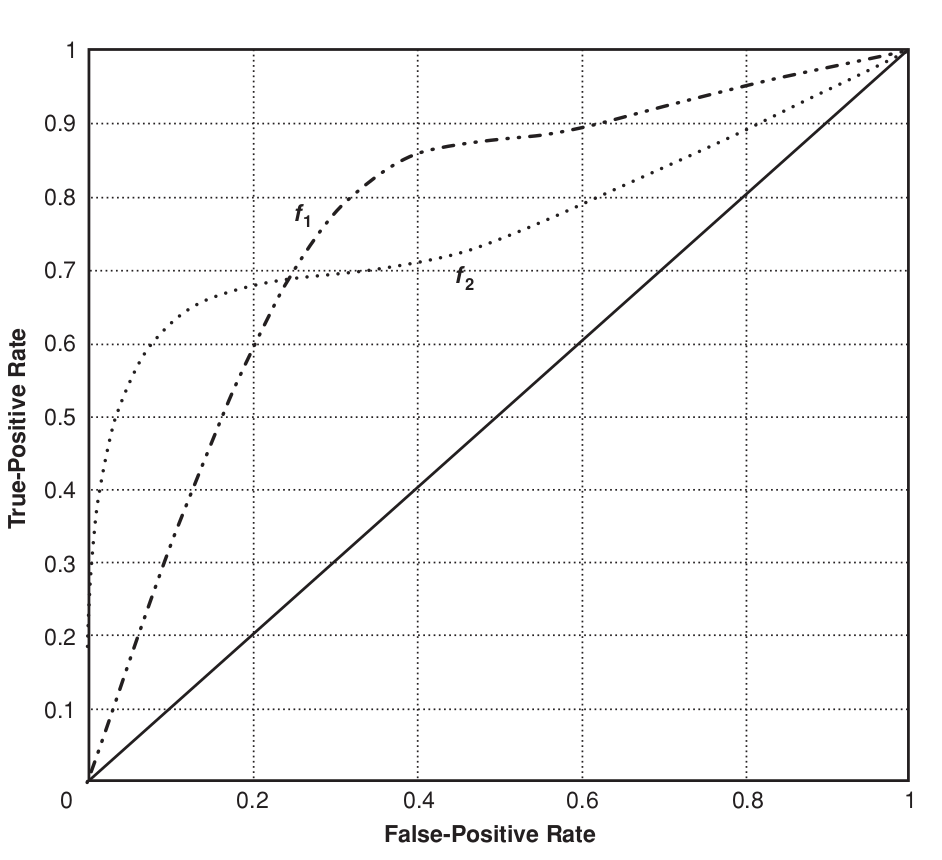
\includegraphics[width=\textwidth]{figure_man/cost-curves-1.png}
    {\tiny Nathalie Japkowicz (2004): Evaluating Learning Algorithms : A
    Classification Perspective. (p. 125)}
  %\end{figure}
\end{column}
\end{columns}

%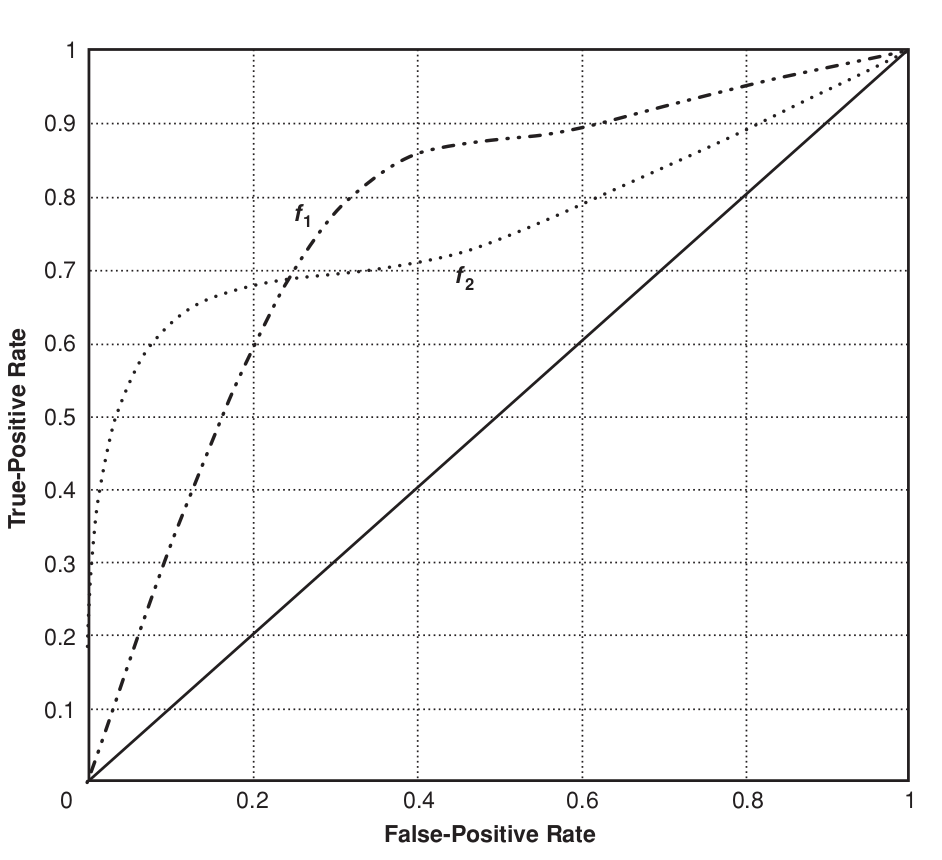
\includegraphics[width=\textwidth]{figure_man/cost-curves-1.png}
% \end{minipage}
% \vspace{1.5 cm}
% {\tiny{Nathalie Japkowicz (2004): Evaluating Learning Algorithms : A Classification Perspective. (p. 125)}}

\end{vbframe}



% ------------------------------------------------------------------------------



\begin{vbframe}{Cost curves}
\small

%Let $\rp = \P(y = 1)$ be the proportion of positive instances.
Simplifying assumption: equal misclassif costs, i.e., $cost_{FN} = cost_{FP}$

$\Rightarrow$ Expected misclassif cost reduces to misclassif error rate

With law of total prob, we write error rate as function of $\rp$:
\begin{align*}
\rho_{MCE}(\rp)
&= (1 - \rp) \cdot \P(\hat y = 1 | y = 0) + \rp \cdot \P(\hat y = 0 | y = 1) \\
&= (1 - \rp) \cdot FPR + \rp \cdot FNR \\
&= (FNR - FPR) \cdot \rp + FPR
\end{align*}
% Can do the same for costs:
% Similarly, expected misclassification costs can be written as a function of $\rp$:
% $$Costs(\rp) = (1 - \rp) \cdot FPR \cdot cost_{FP} + \rp \cdot FNR \cdot cost_{FN}$$
% $$Costs_{norm}(\rp) = \tfrac{(1 - \rp) \cdot FPR \cdot cost_{FP} \; + \; \rp \cdot FNR \cdot cost_{FN}}{(1 - \rp) \cdot cost_{FP} \; + \; \rp \cdot cost_{FN}} \in [0,1]$$

\begin{columns}[T]
% \begin{column}{0.64\textwidth}
% \small
% \begin{itemize}
% \itemsep0em
% % \item $Costs_{norm}$ (normalized costs) is a natural extension of MCE
% \item Denominator = $\max(Costs)$ =  all obs misclassified (i.e., $FPR = FNR = 1$).
% % \item If $cost_{FN} = cost_{FP}$, then $Costs_{norm} = \rho_{MCE}$
% \end{itemize}
% \end{column}
\begin{column}{0.5\textwidth}
% \tiny

%\begin{center}
\centerline{Confusion matrix}
\begin{tabular}{cc|cc}
    & &\multicolumn{2}{c}{True class} \\
    & & $y=1$ & $y=0$  \\
 \hline
    \multirow{2}{*}{\parbox{0.5cm}{Pred. class}}& $\hat y$ = 1     & TP                 & FP\\
    & $\hat y$ = 0 & FN              & TN\\
    %& & P(y = 1) & P(y = 0)
\end{tabular}
\end{column}

% \lz
\begin{column}{0.5\textwidth}
\centerline{Cost matrix}
\begin{tabular}{cc|cc}
    & &\multicolumn{2}{c}{True class} \\
    & & $y=1$ & $y=0$  \\
 \hline
    \multirow{2}{*}{\parbox{0.5cm}{Pred. class}}& $\hat y$ = 1     & 0                 & $cost_{FP}$\\
    & $\hat y$ = 0 & $cost_{FN}$              & 0\\
    %& & P(y = 1) & P(y = 0)
\end{tabular}
%\end{center}

\end{column}
\end{columns}

% \begin{columns}
% \begin{column}{0.5\textwidth}
% {\centering Confusion matrix
% \begin{center}
% \begin{tabular}{cc|cc}
%     & &\multicolumn{2}{c}{True class} \\
%     & & $y=1$ & $y=0$  \\
%  \hline
%     \multirow{2}{*}{\parbox{0.6cm}{Pred.  class}}& $\hat y$ = 1     & TP                 & FP\\
%     & $\hat y$ = 0 & FN              & TN\\
%     %& & P(y = 1) & P(y = 0)
% \end{tabular}
% \end{center}
% }
% \end{column}
% \begin{column}{0.5\textwidth}
% {\centering Cost matrix
% \begin{center}
% \begin{tabular}{cc|cc}
%     & &\multicolumn{2}{c}{True class} \\
%     & & $y=1$ & $y=0$  \\
%  \hline
%     \multirow{2}{*}{\parbox{0.6cm}{Pred.  class}}& $\hat y$ = 1     & 0                 & $cost_{FP}$\\
%     & $\hat y$ = 0 & $cost_{FN}$              & 0\\
%     %& & P(y = 1) & P(y = 0)
% \end{tabular}
% \end{center}
% }
% \end{column}
% \end{columns}


\end{vbframe}

% ------------------------------------------------------------------------------

\begin{vbframe}{Cost curves}

\begin{footnotesize}

\begin{itemize}
  % \item Simplifying assumption: equal misclassification costs, i.e.,
  % $cost_{FN} = cost_{FP}$.
  \item Cost line of a classifier with slope $(FNR - FPR)$ and intercept $FPR$: $$\rho_{MCE}(\rp) = (FNR - FPR) \cdot \rp + FPR$$
  \item Cost curves are point–line duals of ROC curves, i.e., a single classifier is represented by a point in the ROC space and by a line in cost space
\end{itemize}

\end{footnotesize}

\begin{figure}
  \centering
  \scalebox{0.8}{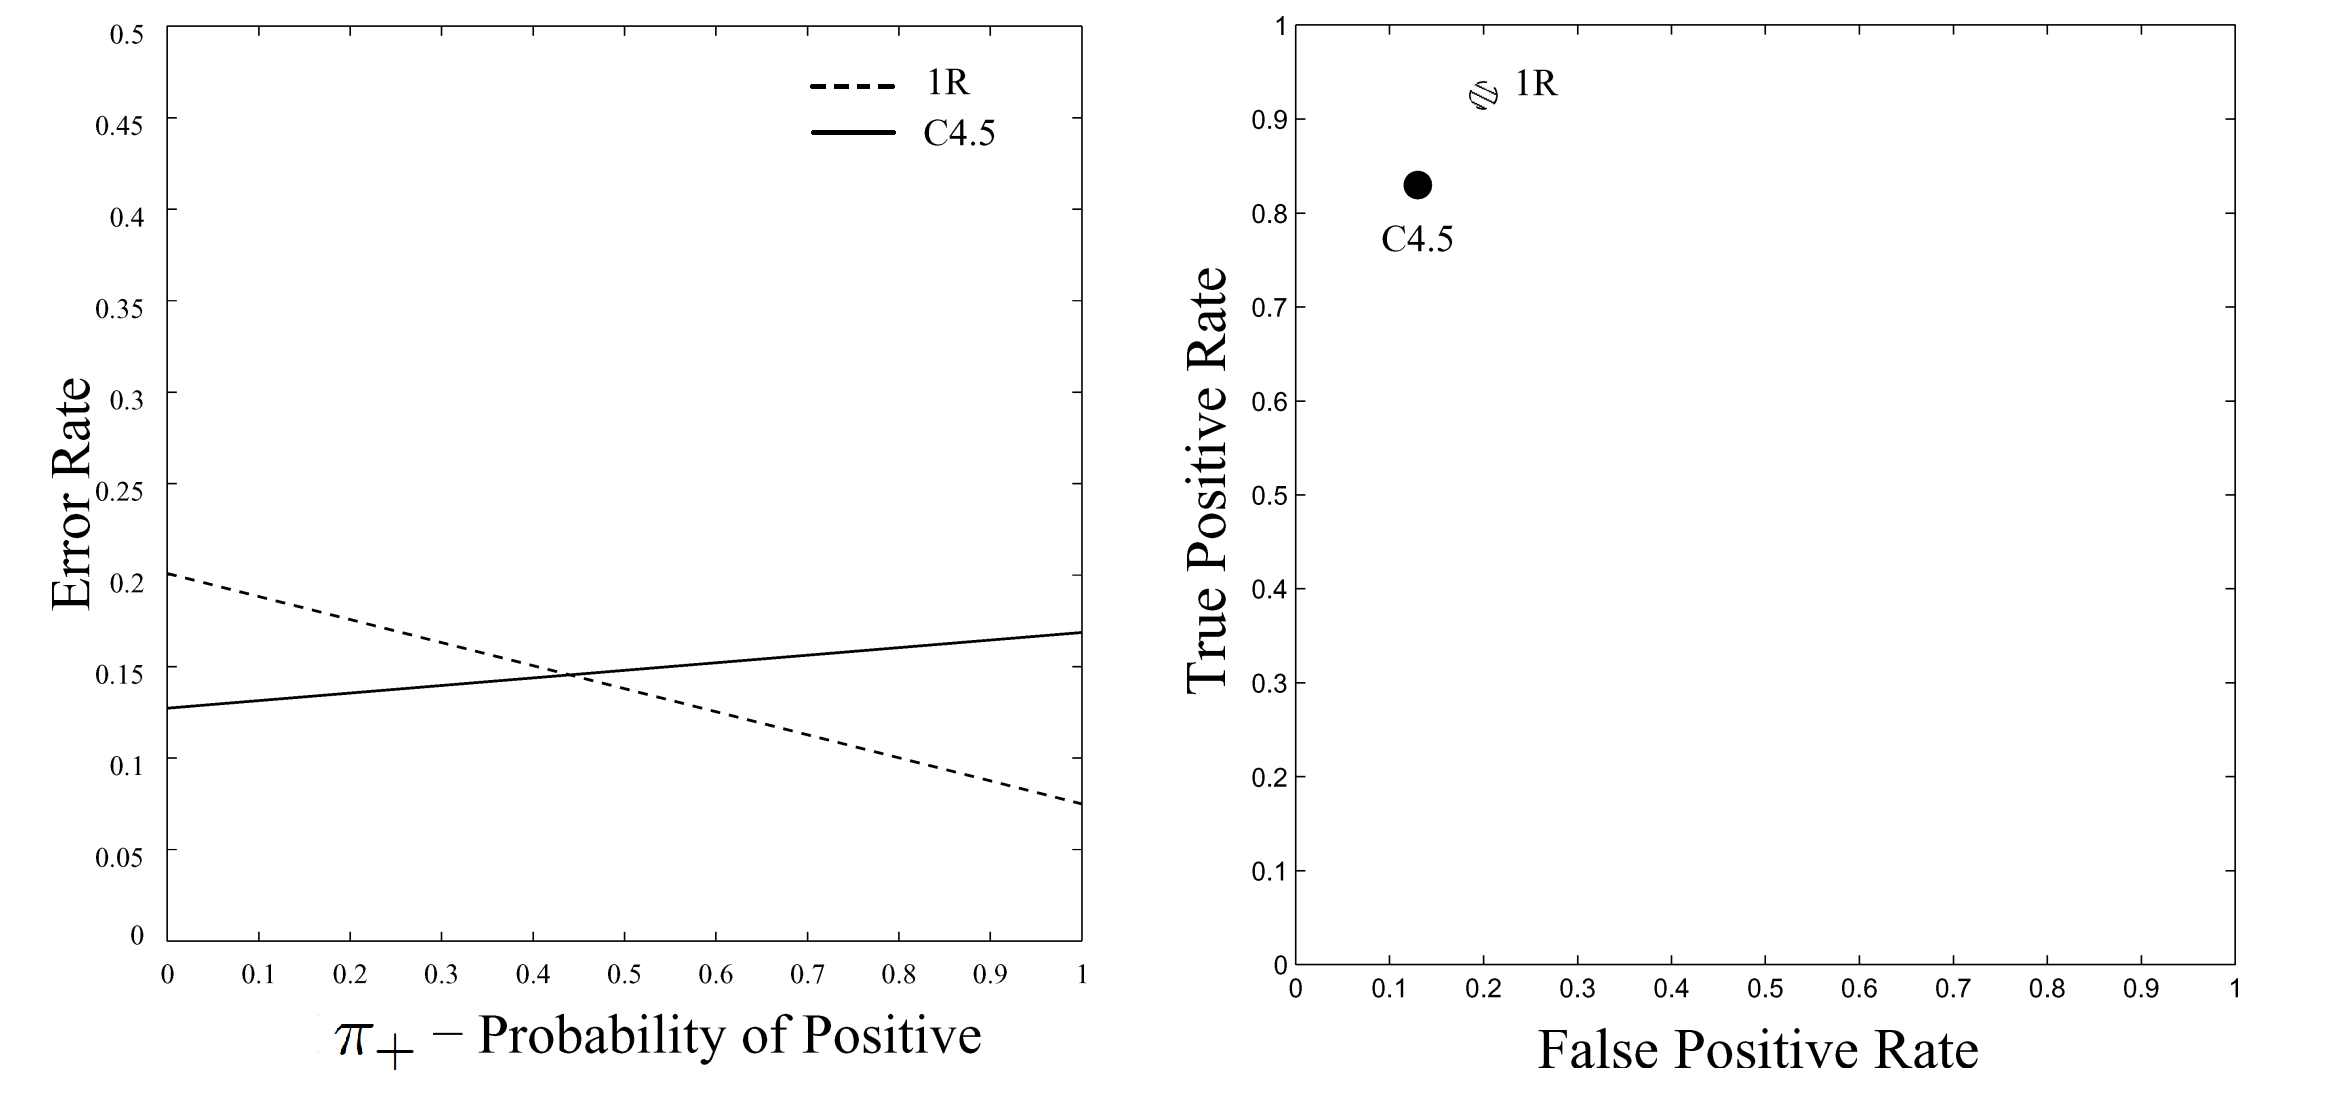
\includegraphics[width=\textwidth]
  {figure_man/cost-curves-0.png}}
  \tiny
  \\Chris Drummond and Robert C. Holte (2006): Cost curves: An improved
  method for visualizing classifier performance. \\Machine Learning, 65, 95-130
  (\href{https://www.semanticscholar.org/paper/Cost-curves\%3A-An-improved-method-for  -visualizing-Drummond-Holte/71708ce984e0896e7383435913547e770572410e}
  {\underline{URL}}).
  % \tiny{\\ Credit: Chris Drummond and Robert C. Holte  \\}
\end{figure}

% {\tiny{Chris Drummond and Robert C. Holte (2006): Cost curves: An improved
% method for visualizing classifier performance. Machine Learning, 65, 95-130.
% \emph{\url{https://www.semanticscholar.org/paper/Cost-curves\%3A-An-improved-method-for-visualizing-Drummond-Holte/71708ce984e0896e7383435913547e770572410e}}}\par}

\end{vbframe}


% ------------------------------------------------------------------------------



\begin{vbframe}{Cost lines}

% \begin{itemize}
  %\item The convex hull of the ROC space is the lower envelope created of all classifier lines in the cost space.
  %\item The misclassification error is plotted as a function of the probability of an observation being from the positive class.
%   \item Functional form of the cost curve of a classifier:
%   $error = (FNR - FPR) \cdot \rp + FPR$ %, \;\;\;$ (Note: $P(+) = \rp$)
% \end{itemize}

Cost line of a classifier with slope $(FNR - FPR)$ and intercept $FPR$:
$$\rho_{MCE}(\rp) = (FNR - FPR) \cdot \rp + FPR$$

\begin{columns}[T]
\begin{column}{0.49\textwidth}

%$error = (\rho_{FNR} - \rho_{FPR}) \cdot \rp + \rho_{FPR}$.
\begin{itemize}
\item Hard classifiers are points (TPR, FPR) in ROC space
\item The cost line of a classifier connects $(\rp, \rho_{MCE})$-points at
$(0, FPR)$ and $(1, 1-TPR)$
\item Classifier 3 always dominates classifier 1
\item Classifier 3 is better than classifier 2 when $\rp < 0.7$
\end{itemize}

\end{column}

\begin{column}{0.49\textwidth}
\centering
Cost lines plot different values of $\rp$ vs. $\rho_{MCE}(\rp)$

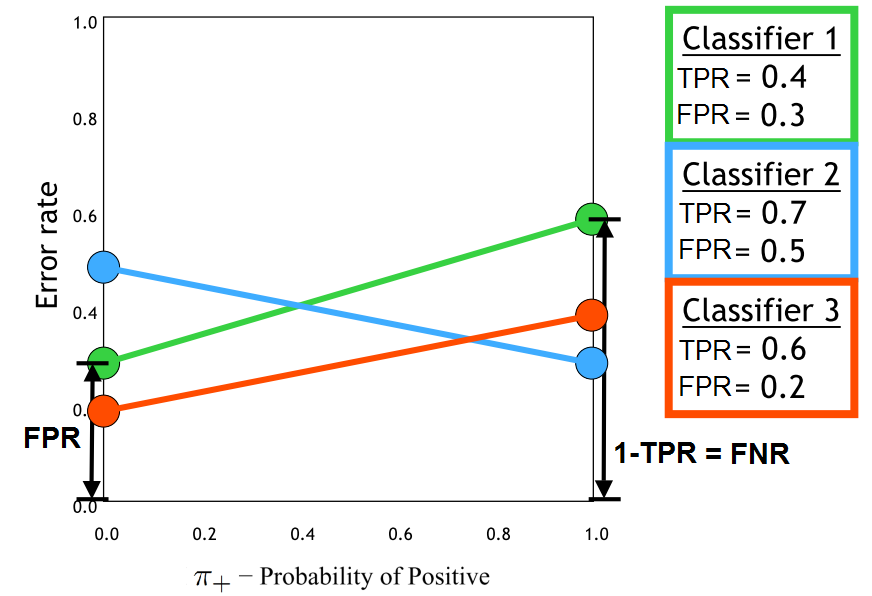
\includegraphics[width=\textwidth]{figure_man/cost-curves-3.png}
\end{column}
\end{columns}
\end{vbframe}

% ------------------------------------------------------------------------------

\begin{frame}{Cost lines - Example}

\begin{footnotesize}

\begin{itemize}
  \item<1-> Horizontal dashed line: worst classifier (100\% error rate for all $\rp$)\\
  $\Rightarrow FNR = FPR = 1$
  \item<1-> x-axis: perfect classifier (0\% error rate for all
  $\rp$) $\Rightarrow FNR = FPR = 0$
  \item<2-> Dashed diagonal lines: trivial classifiers, i.e., ascending diagonal always predicts negative instances ($\Rightarrow FNR = 1$ and $FPR = 0$) and vice versa
  \item<3-> Descending/ascending bold lines:
  two families of classifiers $A$ and $B$ (represented by points in their respective ROC curves)
\end{itemize}

\end{footnotesize}

% Animation: https://docs.google.com/presentation/d/1YWmJeb9etd8-dtwU8jfmJZPbJKoWTuz7CQtNnSEtu54/edit?usp=sharing
\begin{columns}[T]
\begin{column}{0.58\textwidth}
%\begin{center}
\includegraphics<1>[page=1, trim = 45 20 50 45, clip, width=\textwidth]{figure_man/cost-curves.pdf}
\includegraphics<2>[page=2, trim = 45 20 50 45, clip, width=\textwidth]{figure_man/cost-curves.pdf}
\includegraphics<3>[page=3, trim = 45 20 50 45, clip, width=\textwidth]{figure_man/cost-curves.pdf}
%\end{center}
\end{column}
\begin{column}{0.41\textwidth}
\footnotesize
$\rho_{MCE} = (FNR - FPR) \cdot \rp + FPR$
{\centering
\begin{center}
Confusion matrix
\begin{tabular}{cc|cc}
    & &\multicolumn{2}{c}{True class} \\
    & & $y=1$ & $y=0$  \\
 \hline
    \multirow{2}{*}{\parbox{0.6cm}{Pred.  class}}& $\hat y$ = 1     & TP                 & FP\\
    & $\hat y$ = 0 & FN              & TN\\
    %& & P(y = 1) & P(y = 0)
\end{tabular}
\end{center}
}
\end{column}
\end{columns}


%\begin{center}
% \only<1>{\centering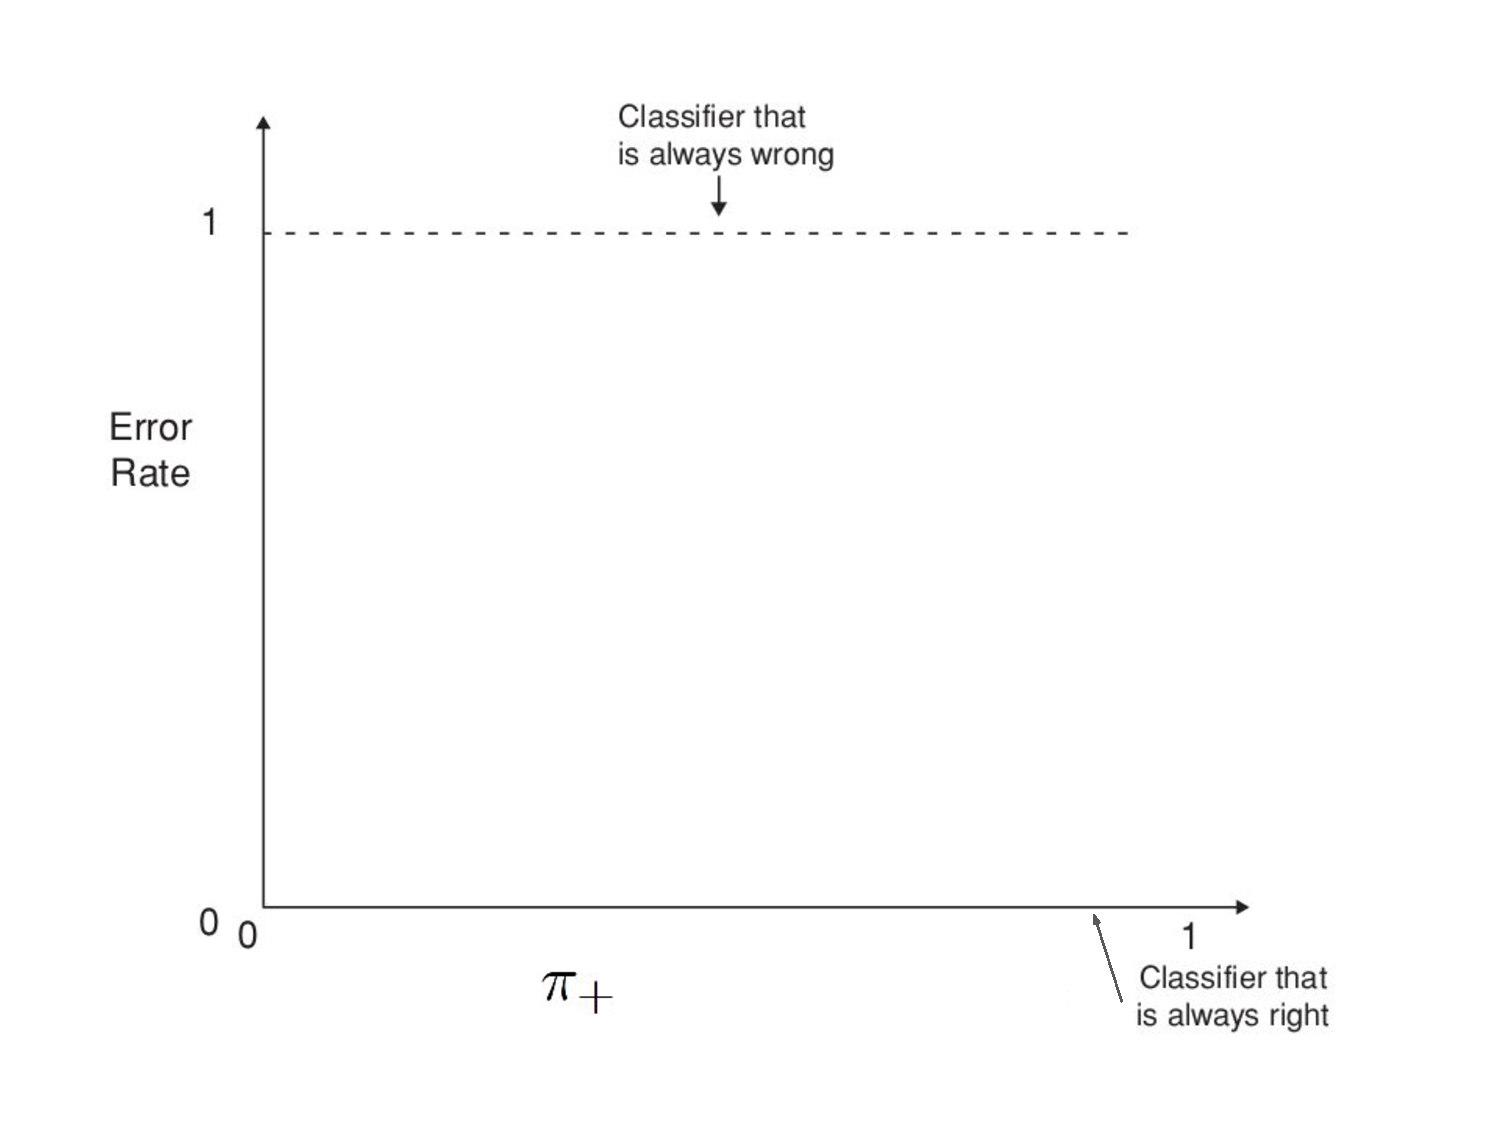
\includegraphics[page=1, width=0.7\textwidth]{figure_man/cost-curves.pdf}}
% \only<2>{\centering\includegraphics[page=2, width=0.7\textwidth]{figure_man/cost-curves.pdf}}
% \only<3>{\centering\includegraphics[page=3, width=0.7\textwidth]{figure_man/cost-curves.pdf}}
  %\tiny{\\ Credit: Nathalie Japkowicz  \\}
%\end{center}

\end{frame}

% ------------------------------------------------------------------------------

% \begin{vbframe}{Cost curves}
%
% \textbf{Example:} In position (0.4, 0.25) B classifier loses its
% performance to one of the A classifiers (point where ROC curves cross). But
% there is no practical information about when classifier A should be used
% over B. In contrast the cost graph tells us that for $0.26 \leq \rp < 0.4$
% classifier B is preferred and for $0.4 \leq \rp < 0.48$ classifier A1 is
% preferred.
%
% \begin{center}
% 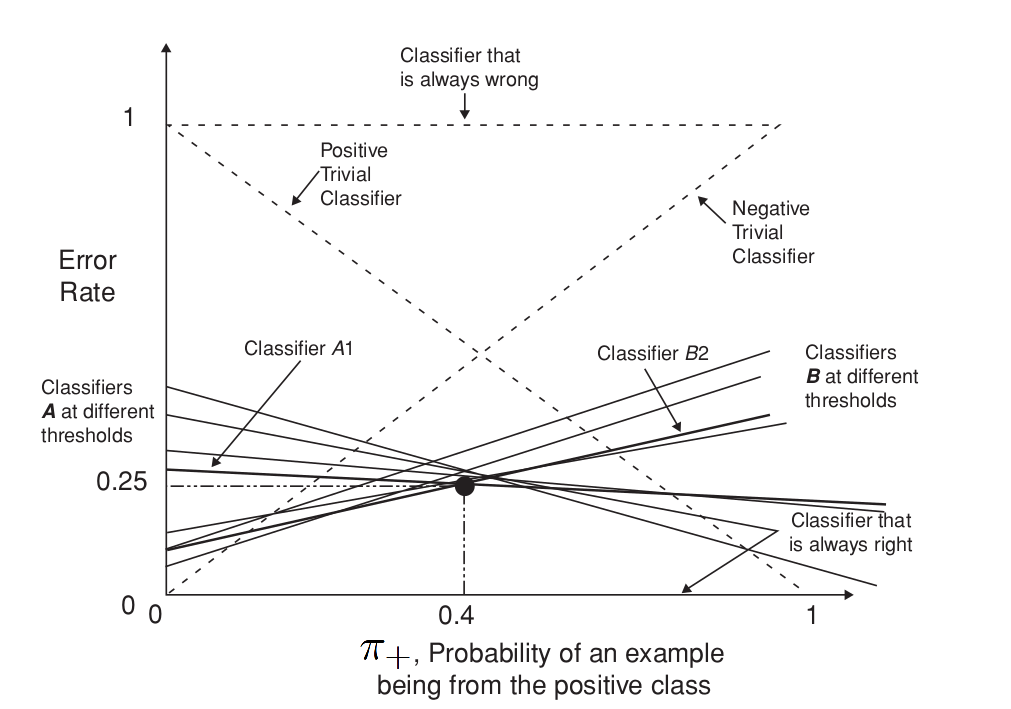
\includegraphics[width=0.5\textwidth]{figure_man/cost-curves-2.png}
% \end{center}
%
% \end{vbframe}

% ------------------------------------------------------------------------------

\begin{frame}{visualize cost curve - lower envelope}

    \begin{itemize}
        \footnotesize
        \item<1-> Left: ROC = TPR $\&$ FPR of a classifier for different prob thresholds
        \item<1-> Right: Corresponding cost lines
        \item<1-> Duality:
        For every ROC point we can construct the CC line, and vice versa.
		\item<4-> \textbf{Cost curve} (right, black) is lower envelope of \textbf{cost lines} \\
		$\hat{=}$ pointwise minimum of error rate (as function of $\rp$)
		%\item The bold curve in the right figure below is the lower envelope of the cost lines
		%\item The lower envelope is a way to visualize the cost curve
	\end{itemize}
  \only<1> {
    \begin{center}
      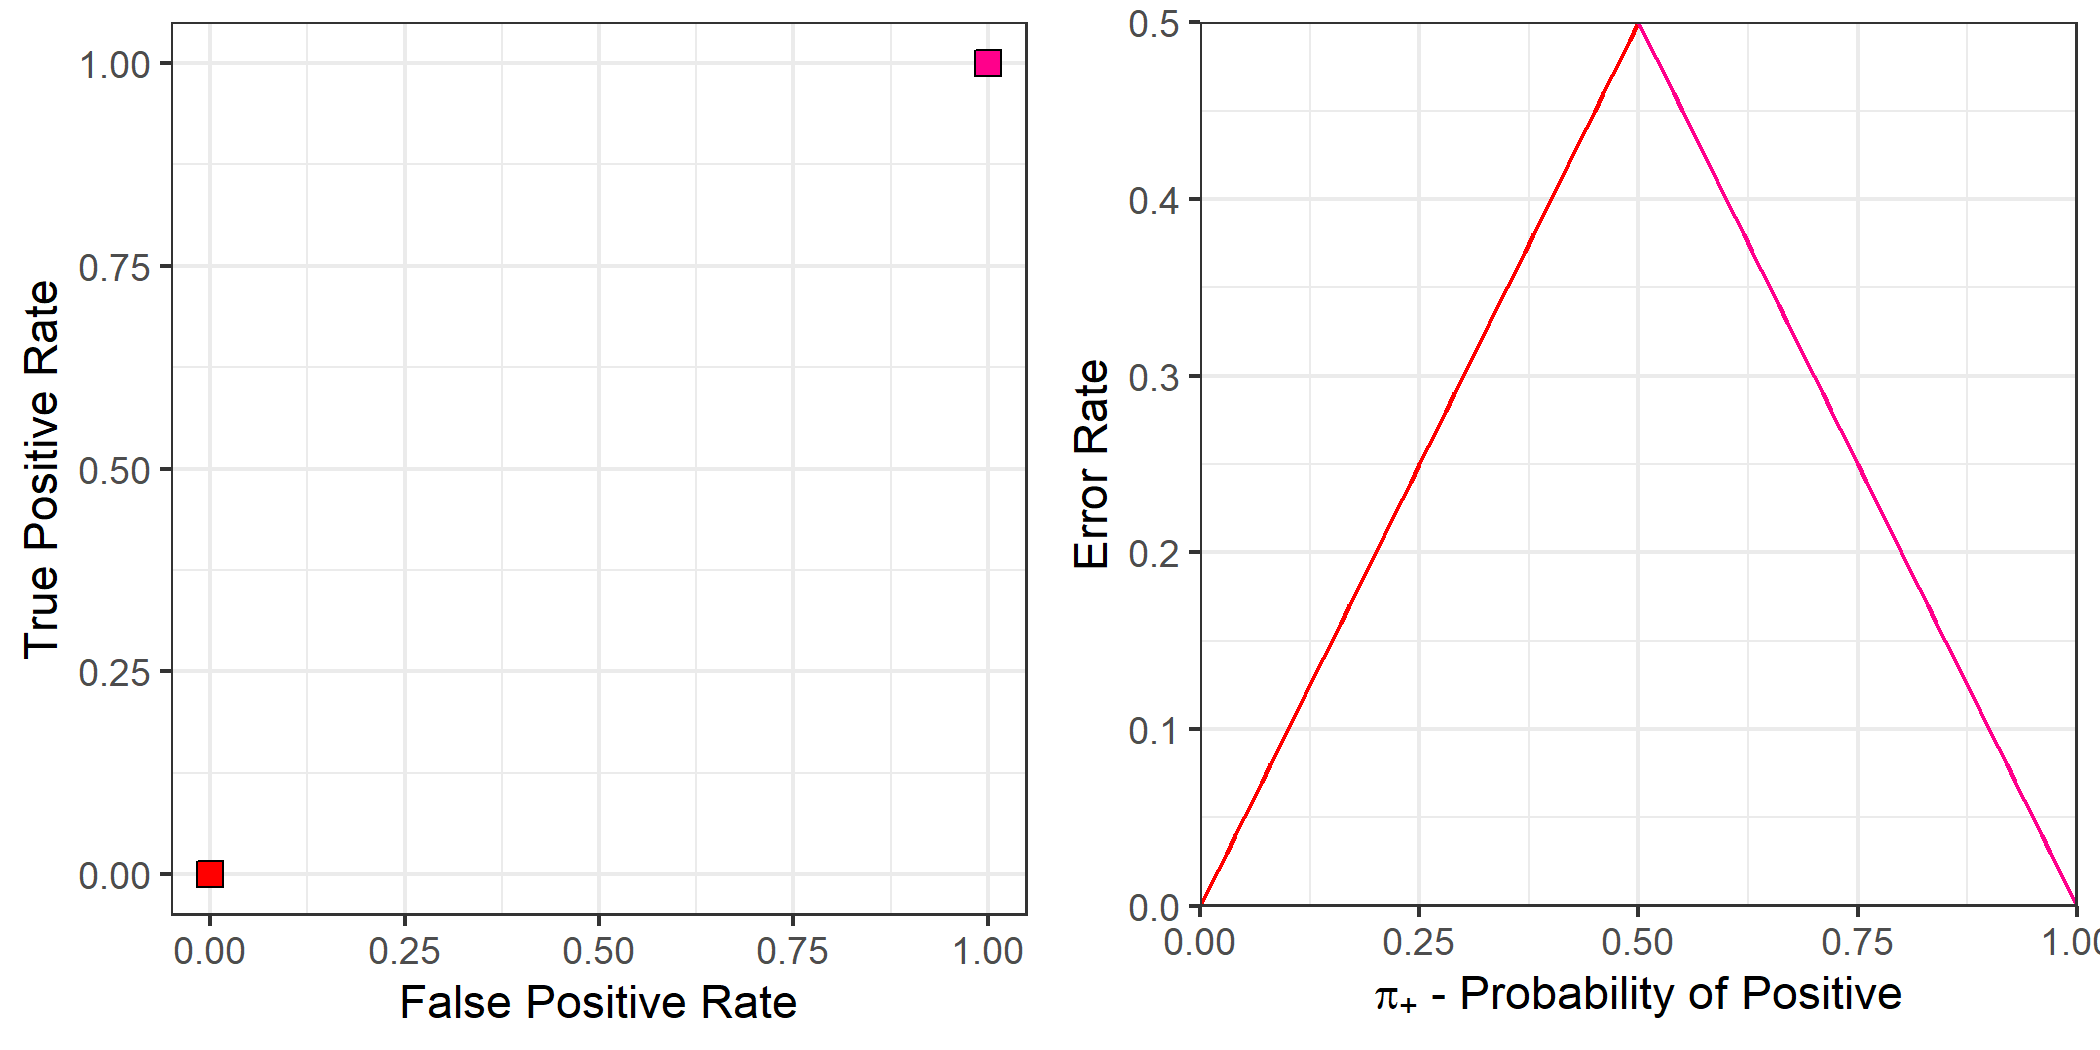
\includegraphics[width=0.8\textwidth]{figure/lower_envelope_1.png}
    \end{center}
  }
  \only<2> {
    \begin{center}
      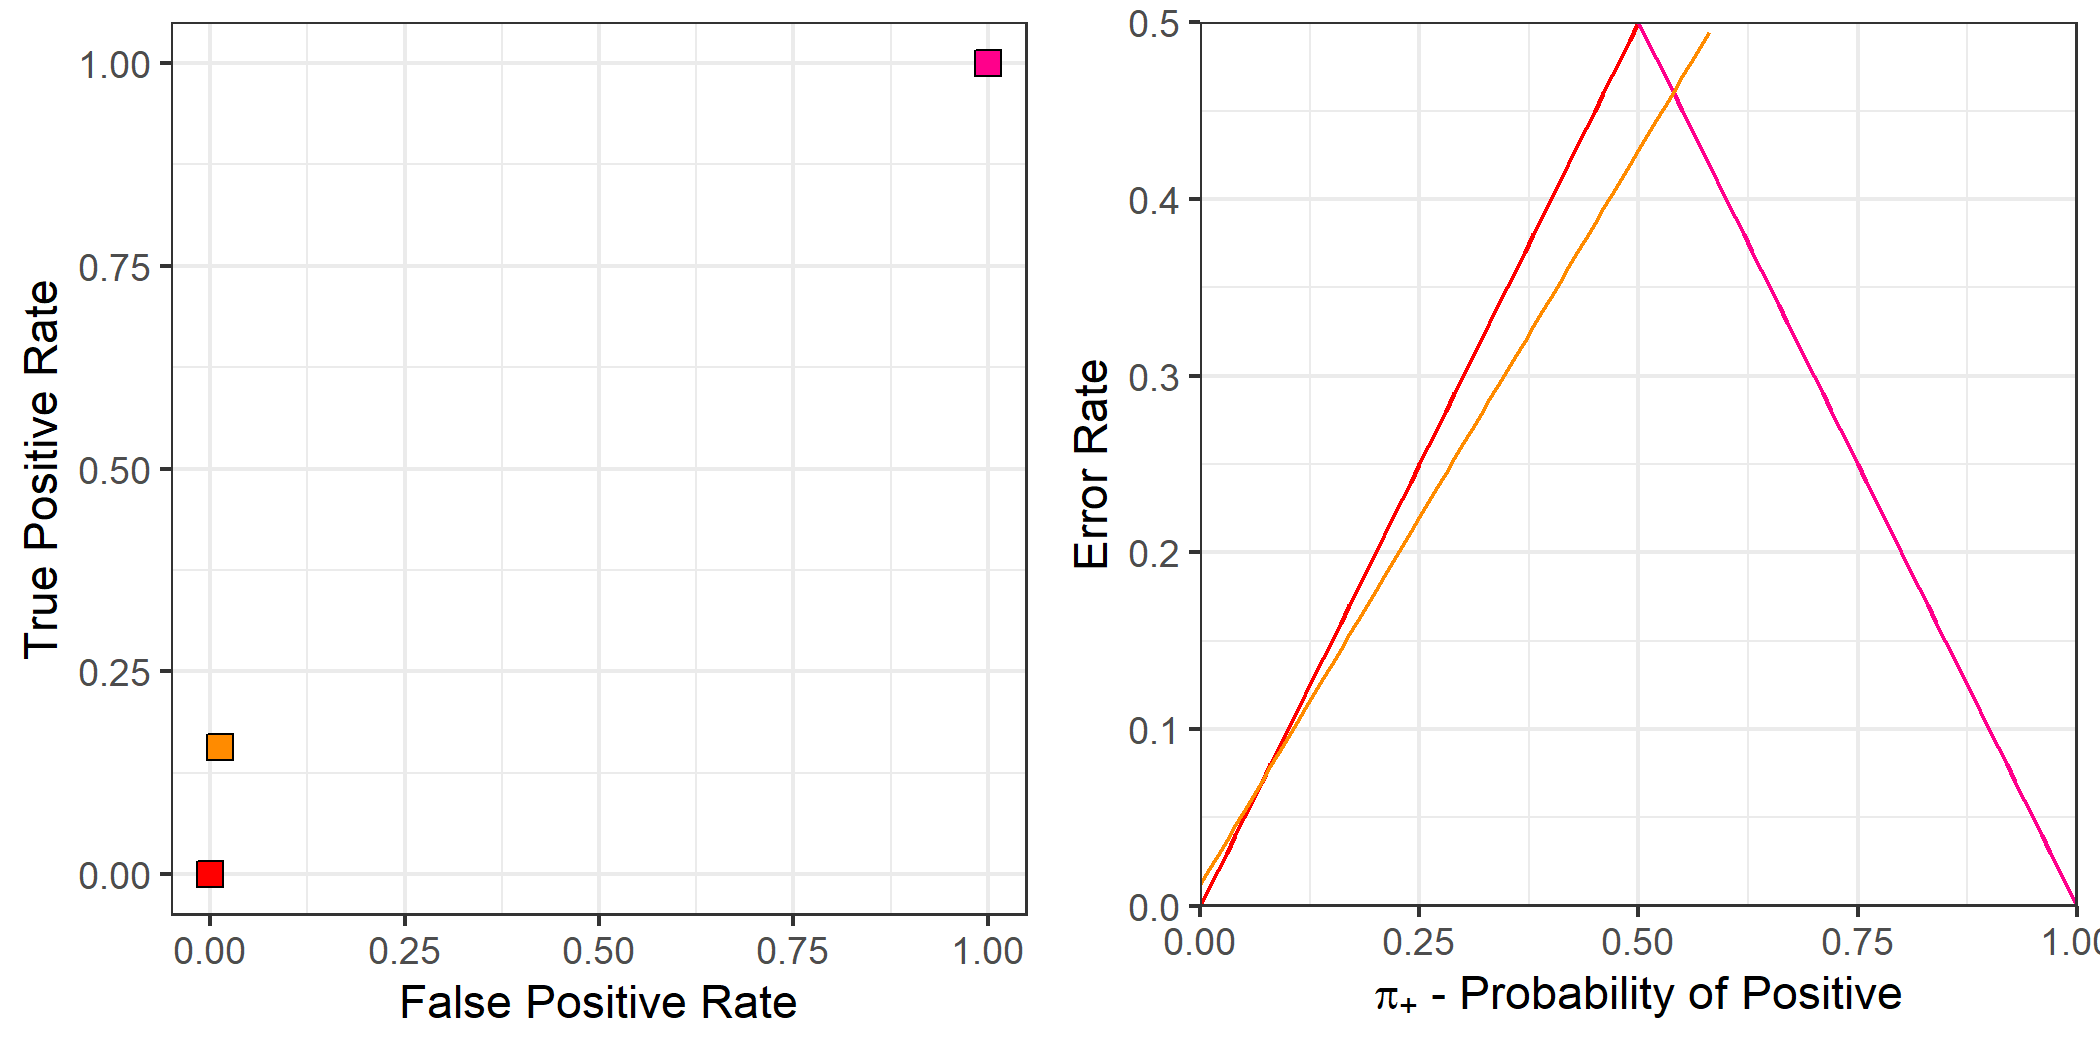
\includegraphics[width=0.8\textwidth]{figure/lower_envelope_2.png}
    \end{center}
  }
  \only<3> {
    \begin{center}
      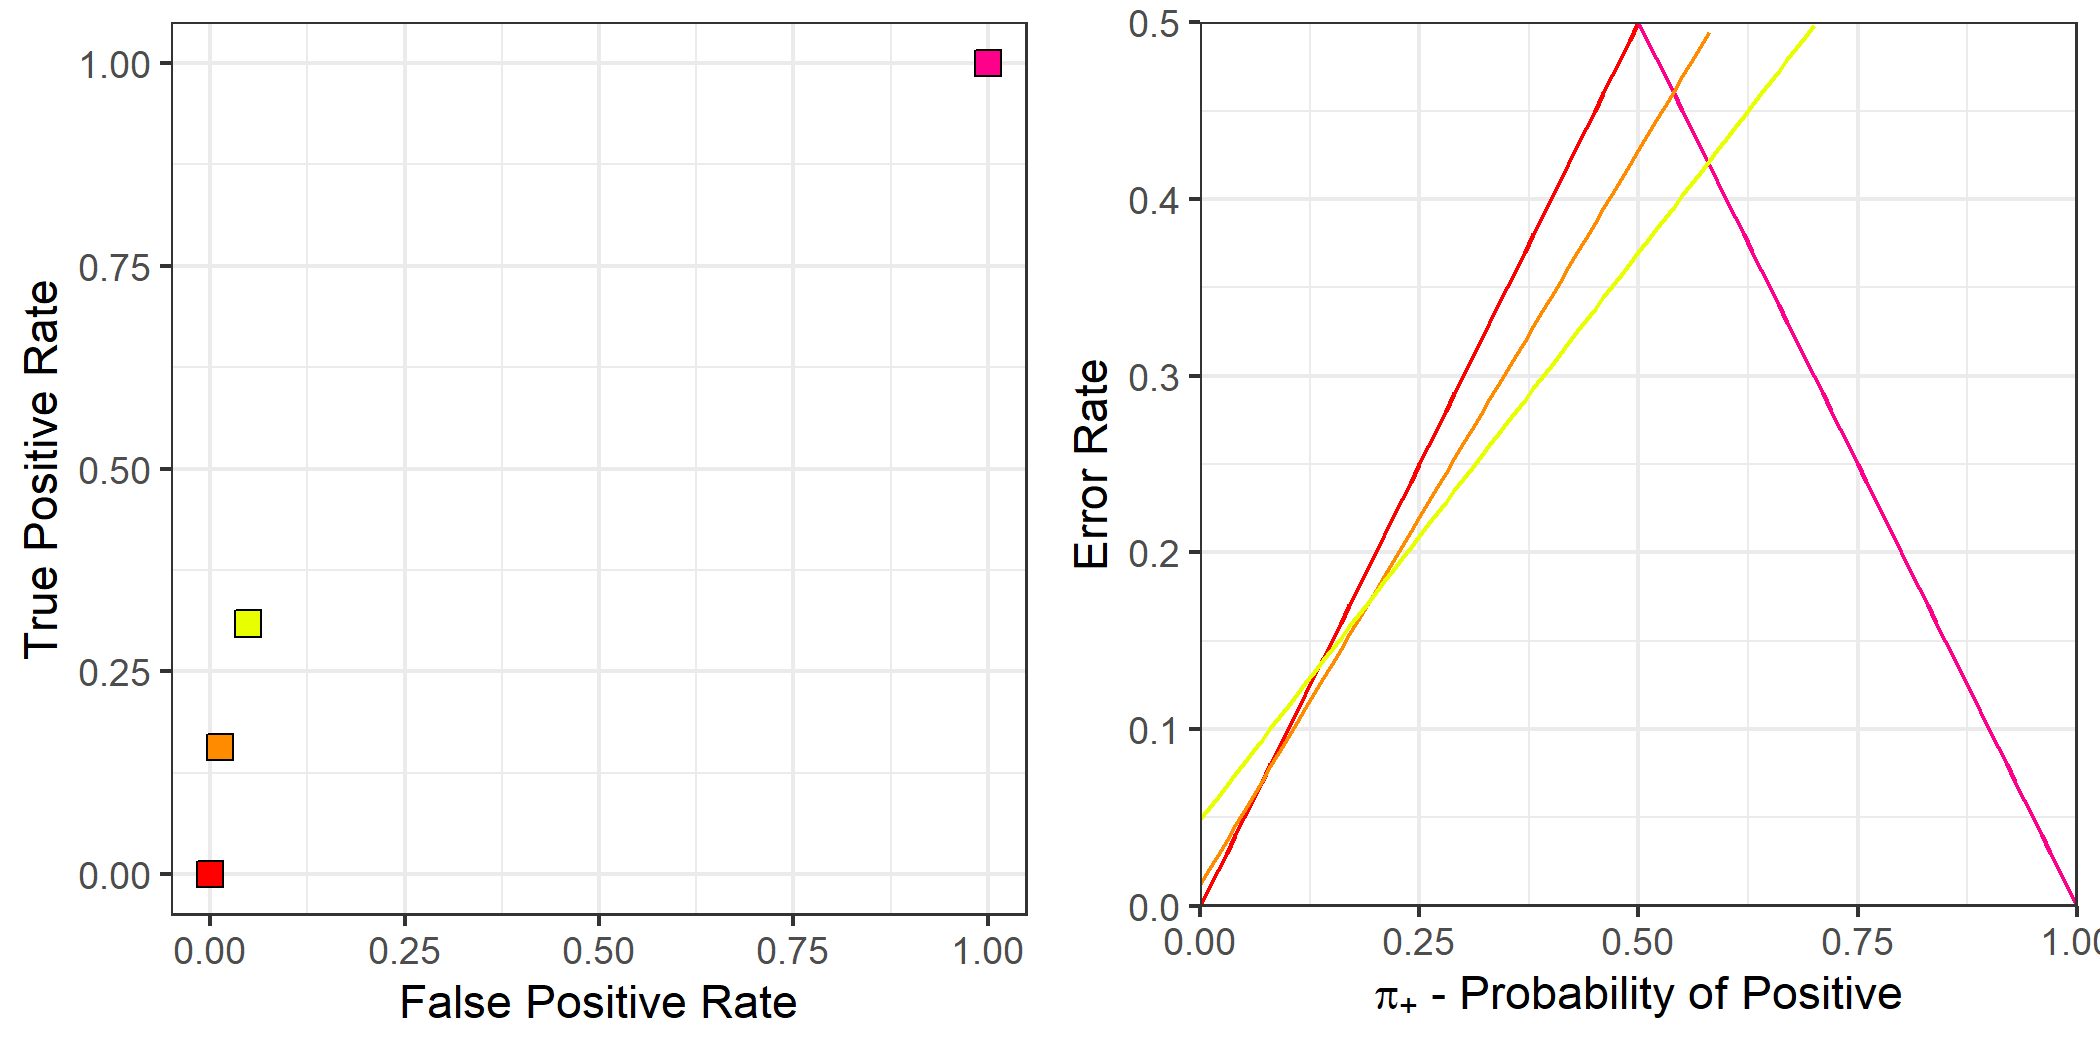
\includegraphics[width=0.8\textwidth]{figure/lower_envelope_3.png}
    \end{center}
  }
  % \only<4> {
  %   \begin{center}
  %     \includegraphics[width=0.8\textwidth]{figure/lower_envelope_4.png}
  %   \end{center}
  % }
  % \only<5> {
  %   \begin{center}
  %     \includegraphics[width=0.8\textwidth]{figure/lower_envelope_5.png}
  %   \end{center}
  % }
  % \only<6> {
  %   \begin{center}
  %     \includegraphics[width=0.8\textwidth]{figure/lower_envelope_6.png}
  %   \end{center}
  % }
  % \only<7> {
  %   \begin{center}
  %     \includegraphics[width=0.8\textwidth]{figure/lower_envelope_7.png}
  %   \end{center}
  % }
  % \only<8> {
  %   \begin{center}
  %     \includegraphics[width=0.8\textwidth]{figure/lower_envelope_8.png}
  %   \end{center}
  % }
  % \only<9> {
  %   \begin{center}
  %     \includegraphics[width=0.8\textwidth]{figure/lower_envelope_9.png}
  %   \end{center}
  % }
  % \only<10> {
  %   \begin{center}
  %     \includegraphics[width=0.8\textwidth]{figure/lower_envelope_10.png}
  %   \end{center}
  % }
  \only<4> {
    \begin{center}
      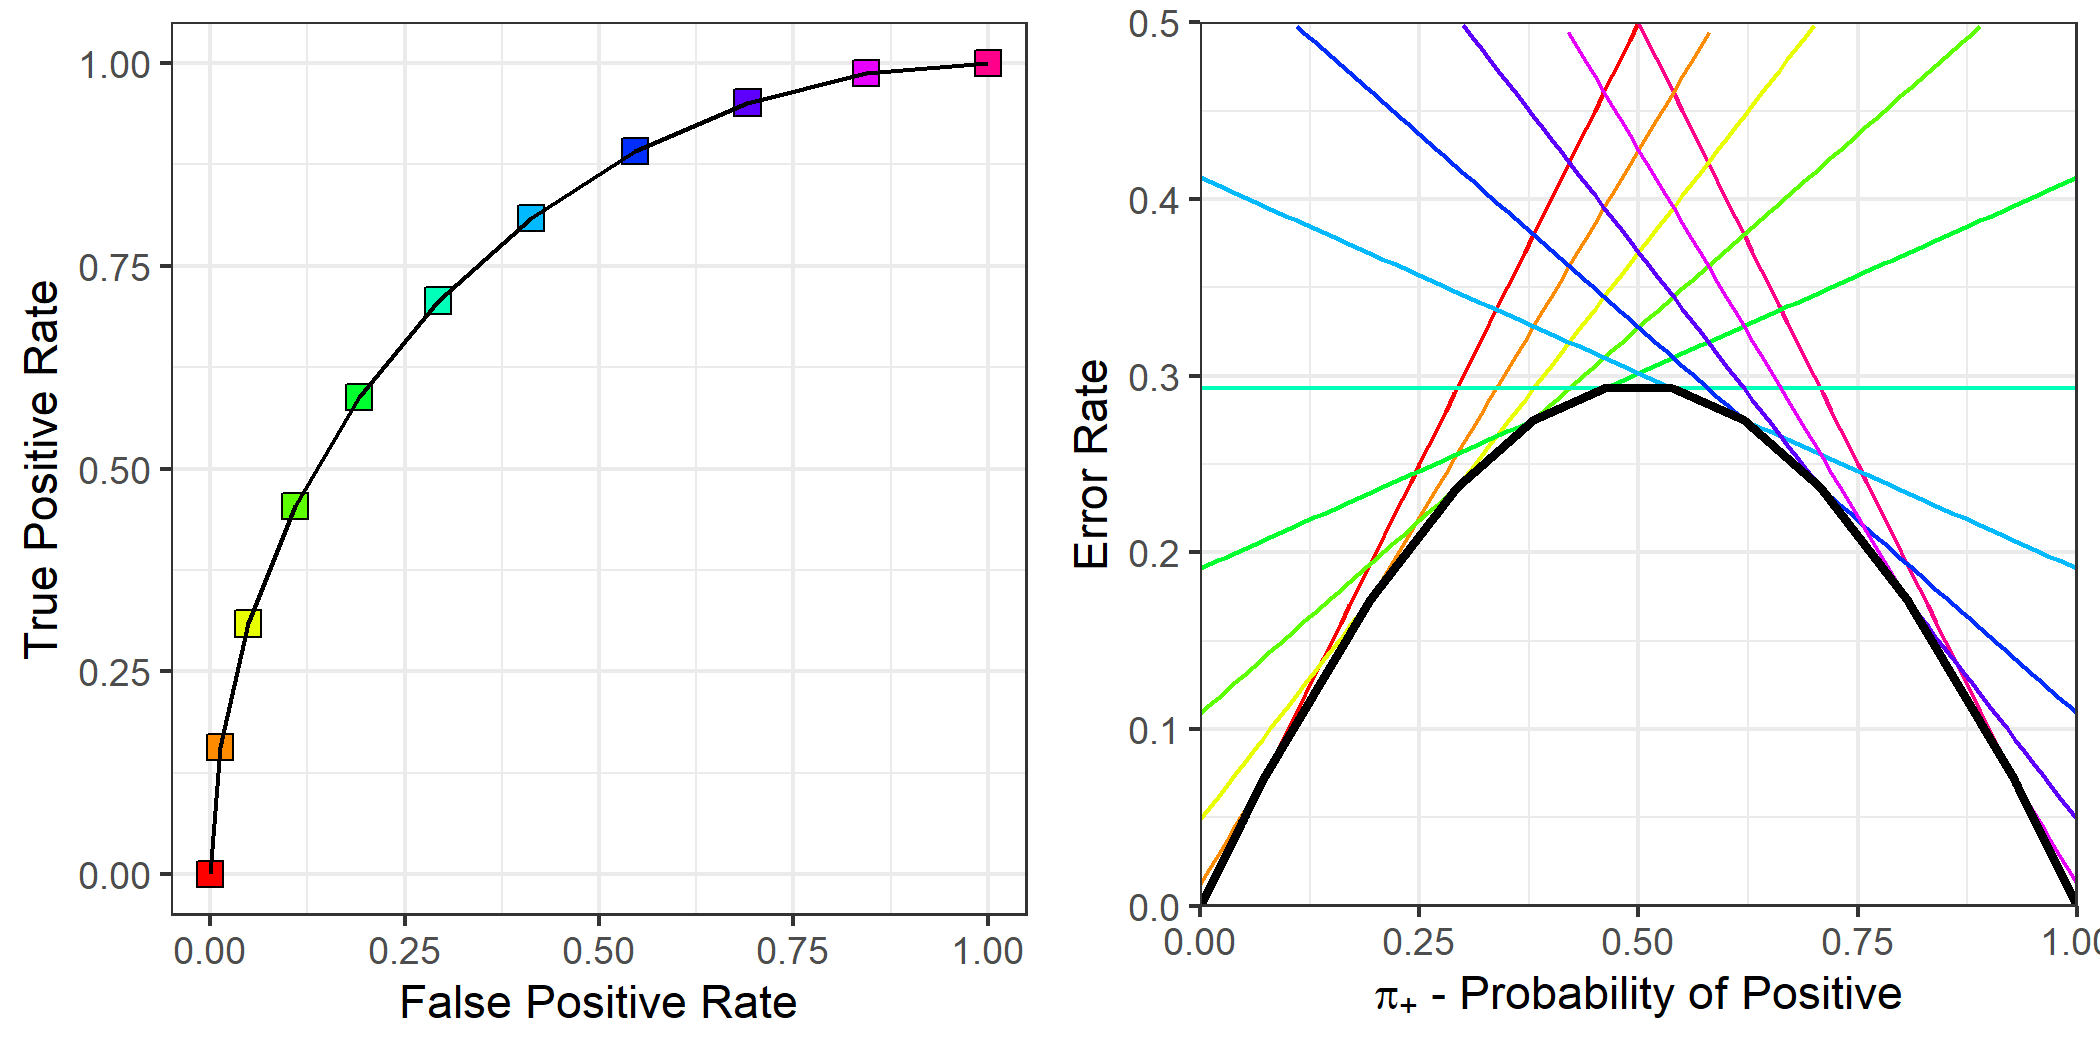
\includegraphics[width=0.8\textwidth]{figure/lower_envelope_11.png}
    \end{center}
  }

\end{frame}

% ------------------------------------------------------------------------------


% ------------------------------------------------------------------------------

% \begin{vbframe}{ROC curves vs. cost curves}
% The general form is as follows:
%
% \vspace{-0.5cm}
% \begin{center}
% \begin{equation*}
% NEC = \text{FNR} \cdot P_C[+] + \text{FPR} \cdot (1 - P_C[+]),
% \end{equation*}
% \end{center}
%
% \begin{itemize}
% \item FNR/FPR are false-negative rate and false-positive rate respectively and
% $P_C[+]$, the probability cost function (modified version of $P[+]$ that takes costs into
% consideration).
%
% \vspace{-0.5cm}
% \begin{center}
% \begin{equation*}
% P_C[+] = \frac{P[+] \cdot C[+|-]}{P[+] \cdot C[+|-] + P[-] \cdot C[-|+]},
% \end{equation*}
% \end{center}
%
% \item $C[+|-]$ and $C[-|+]$ represent the cost of predicting a positive when the
% instance is actually negative and vice versa and $P[-]$ as the probability of
% being in the negative class.
% \end{itemize}
% \end{vbframe}

% ------------------------------------------------------------------------------
\endlecture
\end{document}
